%%%%%%%%%%%%%%%%%%%%%%%%%%%%%%%%%%%%%%%%%
% Journal Article
% LaTeX Template
% Version 1.3 (9/9/13)
%
% This template has been downloaded from:
% http://www.LaTeXTemplates.com
%
% Original author:
% Frits Wenneker (http://www.howtotex.com)
%
% License:
% CC BY-NC-SA 3.0 (http://creativecommons.org/licenses/by-nc-sa/3.0/)
%
%%%%%%%%%%%%%%%%%%%%%%%%%%%%%%%%%%%%%%%%%

%----------------------------------------------------------------------------------------
%	PACKAGES AND OTHER DOCUMENT CONFIGURATIONS
%----------------------------------------------------------------------------------------

\documentclass[twoside]{article}

\usepackage{lipsum} % Package to generate dummy text throughout this template

\usepackage[sc]{mathpazo} % Use the Palatino font
\usepackage{amsmath}
\usepackage[T1]{fontenc} % Use 8-bit encoding that has 256 glyphs
\linespread{1.05} % Line spacing - Palatino needs more space between lines
\usepackage{microtype} % Slightly tweak font spacing for aesthetics

\usepackage[hmarginratio=1:1,top=32mm,columnsep=20pt]{geometry} % Document margins
\usepackage{multicol} % Used for the two-column layout of the document
\usepackage[hang, small,labelfont=bf,up,textfont=it,up]{caption} % Custom captions under/above floats in tables or figures
\usepackage{booktabs} % Horizontal rules in tables
\usepackage{float} % Required for tables and figures in the multi-column environment - they need to be placed in specific locations with the [H] (e.g. \begin{table}[H])
\usepackage{hyperref} % For hyperlinks in the PDF

\usepackage{lettrine} % The lettrine is the first enlarged letter at the beginning of the text
\usepackage{paralist} % Used for the compactitem environment which makes bullet points with less space between them

\usepackage{abstract} % Allows abstract customization
\renewcommand{\abstractnamefont}{\normalfont\bfseries} % Set the "Abstract" text to bold
\renewcommand{\abstracttextfont}{\normalfont\small\itshape} % Set the abstract itself to small italic text

\usepackage{float}% Places a thin box around figures
\floatstyle{boxed} 
\restylefloat{figure}
\usepackage{graphicx}


\usepackage{titlesec} % Allows customization of titles
\renewcommand\thesection{\Roman{section}} % Roman numerals for the sections
\renewcommand\thesubsection{\Roman{subsection}} % Roman numerals for subsections
\titleformat{\section}[block]{\large\scshape\centering}{\thesection.}{1em}{} % Change the look of the section titles
\titleformat{\subsection}[block]{\large}{\thesubsection.}{1em}{} % Change the look of the section titles

\usepackage{fancyhdr} % Headers and footers
\pagestyle{fancy} % All pages have headers and footers
\fancyhead{} % Blank out the default header
\fancyfoot{} % Blank out the default footer
\fancyhead[C]{Heavy Photon Search Collaboration Note $\bullet$ August 2015} % Custom header text
\fancyfoot[RO,LE]{\thepage} % Custom footer text

%----------------------------------------------------------------------------------------
%	TITLE SECTION
%----------------------------------------------------------------------------------------

\title{\vspace{-15mm}\fontsize{24pt}{10pt}\selectfont\textbf{HPS Ecal Timing Calibration for the Spring 2015 Engineering Run}} % Article title

\author{
\large
\textsc{Holly Szumila-Vance}\thanks{Many thanks for the helpful discussions and advice of Stepan Stepanyan, Larry Weinstein, and Nathan Baltzell}\\[2mm] % Your name
\normalsize Old Dominion University\\ % Your institution
\normalsize \href{mailto:hszumila@jlab.org}{hszumila@jlab.org} % Your email address
\vspace{-5mm}
}
\date{}

%----------------------------------------------------------------------------------------

\begin{document}

\maketitle % Insert title

\thispagestyle{fancy} % All pages have headers and footers

%----------------------------------------------------------------------------------------
%	ABSTRACT
%----------------------------------------------------------------------------------------

\begin{abstract}

\noindent % \lipsum[1] % Dummy abstract text
This note describes the timing calibration of the HPS Ecal during the Spring 2015 engineering run. In this calibration, the accelerator RF signal was used to fine tune measured time offsets for each crystal. By studying the timing of hits within a cluster, a time walk correction was found that can be used to improve clustering in offline reconstruction. The main HPS two-cluster trigger enabled studying of large time offsets in crystals. While the FADC250s sample a signal every 4 ns, it was found that after timing offsets and time walk corrections were accounted for, the two cluster resolution for well-correlated pairs is on the order of 480 ps which can be used to reduce accidentals. 

\end{abstract}

%----------------------------------------------------------------------------------------
%	ARTICLE CONTENTS
%----------------------------------------------------------------------------------------

\begin{multicols}{2} % Two-column layout throughout the main article text

\section{Introduction}

%\lettrine[nindent=0em,lines=3]{T} 
The HPS Ecal's primary purpose is for triggering events for read out. Offline, timing is important to the success of HPS as it can be used to reduce accidentals in two-cluster events and improve cluster reconstruction. The two-cluster pairs trigger is the primary trigger used by HPS in order to find correlated $e^+e^-$ events for reconstructing the invariant mass and analyzing the spectrum for a possible Heavy Photon signal.\\ \indent The PbWO$_4$ crystals of the Ecal are readout using FADC250s which sample the input signals at 250 MHz, or every 4 ns. The accelerator RF signal enters Hall B at 499 MHz and is sampled every 80 signals ~\cite{Kazimi}. The RF signal is  split in the hall and readout by two FADC250 channels. All data taken during the Spring 2015 running was taken using the FADC250 Mode 1 which corresponds to the full raw waveform read out. In offline reconstruction, each pulse is fit using a 3-pole function that is detailed in ~\cite{Baltzell}. The time for a hit is obtained from the parameters in this fitting method. Clusters are formed by searching for seed hits (highest energy crystal with all surrounding crystals lower in energy) and adding hits that surround the seed hits. Clustering can be improved with detailed studies of timing so that out of time hits from different events are not added to clusters. 
 
%------------------------------------------------

\section{Methods}

Several techniques were used in conjunction with each other to find time offsets for each crystal and to study time walk and resolution as a function of energy.\\ \indent The first step uses the remainder of the time difference between the RF signal and crystal signal to fine tune the time offsets. Because the modulo of the RF signal time is used, the resultant signals are tuned to increments of 2 ns (corresponding the RF signal frequency).\\ \indent The second step looks for the gross time offsets in increments of 2 ns by using the time difference between two well-correlated clusters in an event. The time walk was studied after removing individual crystal time offsets by comparing the hit times in a cluster against the seed time as a function of the hit energies.\\
\subsection{RF Signal}
\subsubsection{Determining the RF signal time}
	In order to use the RF signal to fine tune the offsets for each crystal, it was first necessary to develop a method to consistently read off the RF time for a pulse. Because the RF signal was split between two different FADC channels, the optimal method for reading off the time should minimize the width in the time difference distribution between the two RF signals. Due to the uniformity of the rise of the RF signal, a straight line fit to the leading edge of the signal was chosen.\\
\begin{figure}[H]
  \centering
      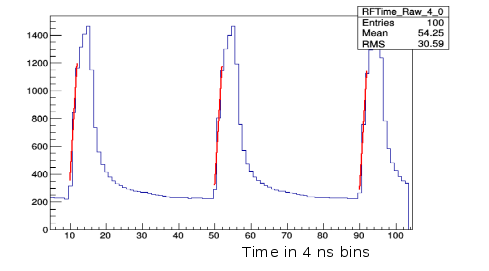
\includegraphics[width=0.5\textwidth]{rfFitting.png}
  \caption{Straight line fit to the leading edge of the RF signal.}
  \label{rfsignal}
\end{figure}	
Since the RF signal is sampled one of every 80 signals going into the hall, each event has two or three RF signals in the readout channel. The window size used for readout is 400 ns and can be seen in Figure \ref{rfsignal}. In order to avoid complications when fitting the signal at the start or end of the window, the second signal in each event was chosen for the timing calibration. After identifying the peak bin (4 ns per bin), the pedestal was calculated by averaging the values in 4 bins occurring at 6 to 9 bins prior to the peak. The threshold used in selecting the fitting points was found by calculating the $1/3$ height between the averaged pedestal and the peak. The points for the straight line fit were then chosen as the last point below this threshold and the next two points above the threshold as can be seen in Figure \ref{rfsignal}. These points were chosen due to the linear uniformity of the pulse away from the peak bin. The time that was used from this fit was at the half height between the pedestal and the peak. This combination of parameters minimized the width of the time difference distribution between the RF signals in the two FADC channels as shown in Figure \ref{rfresolution}. This width of 24 ps corresponds to the internal resolution of the system.\\ 
\begin{figure}[H]
  \centering
      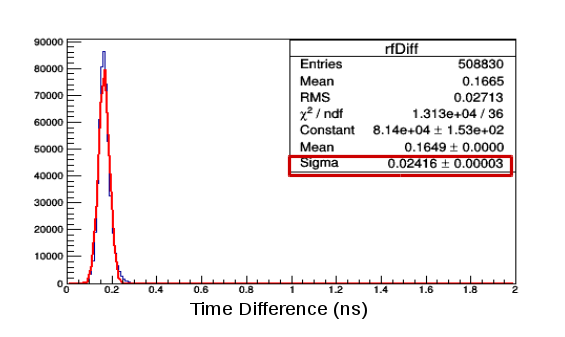
\includegraphics[width=0.5\textwidth]{rfRes.png}
  \caption{Time difference between the RF signal in the two different FADC channels.}
  \label{rfresolution}
\end{figure}

\subsubsection{Individual crystal fine time offsets}
	For each event, the time difference between the hit in a cluster ($t_{hit}$) and the RF signal time ($t_{RF}$) was histogrammed for each crystal. 
\begin{equation}
\label{eq:timediff}
\Delta t = t_{hit}-t_{RF} 
\end{equation}	
The beam structure is apparent as can be seen in Figure \ref{fig:spectra}. Because the RF signal time occurs with a frequency of 499 MHz, Equation \ref{eq:toff} was used to plot the distribution for finding the fine time offset per crystal.  \\
\begin{equation}
\label{eq:toff}
\Delta t_{fine} = fmod(\Delta t+N\times 2.004)-1.002 \textit{ ns}
\end{equation}
We fit the $\Delta t_{fine}$ spectrum for each peak with a Gaussian and used the peak position as a time offset to iteratively correct the timing (see \ref{fig:spectra2}). Generally, the first iteration shifts the peak by simply choosing the maximum bin so that the distribution is entirely contained between -1 to 1 ns. The next two iterations apply a fit to the peak to obtain the mean value until there are no longer significant deviations from zero.    
\begin{figure}[H]
  \centering
      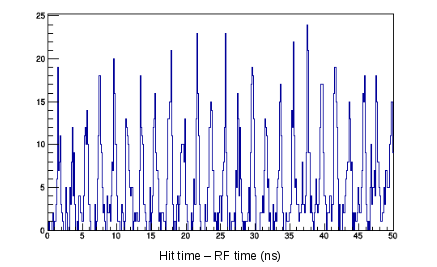
\includegraphics[width=0.5\textwidth]{crystalSpectra.png}
  \caption{Difference in time between a single crystal hit and the RF time.}
  \label{fig:spectra}
\end{figure}
\begin{figure}[H]
  \centering
      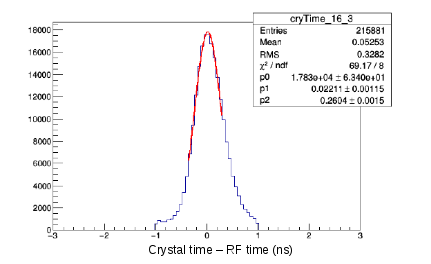
\includegraphics[width=0.5\textwidth]{crystalSpectra2.png}
  \caption{Fine time offset after second iteration for an individual crystal.}
    \label{fig:spectra2}
\end{figure}
\subsection{Two Cluster Pairs}
In order to find the large time offsets (in increments of 2 ns due to the accelerator RF frequency), two cluster pairs events were studied. The time of a cluster was found to be the time of the seed hit, or highest energy hit. Comparison studies were done to check if a hit energy weighted distribution could improve cluster time, but these calculations made no significant difference as the seed hit energy dominates the time distribution and the results come out to be the same as simply using the time of the seed hit. By searching through events that were triggered by a pair of well-correlated clusters, the time difference between these pairs could be plotted per seed hit crystal. The resultant distributions occur at 2 ns intervals as seen in Figure \ref{pairsprocedure}. 
\begin{figure}[H]
  \centering
      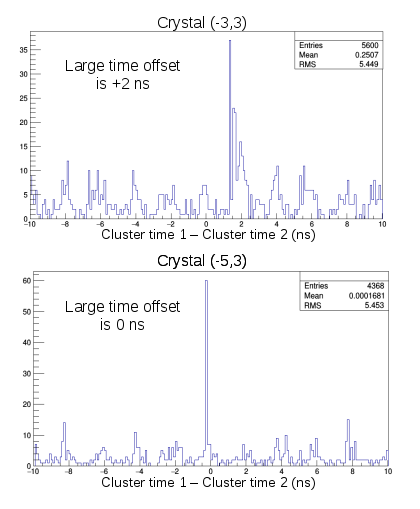
\includegraphics[width=0.5\textwidth]{pairsProcedure.png}
  \caption{Time difference between the seed hits of two well-correlated clusters after RF calibration. The top and bottom plots show events where crystal $(-3,3)$ and crystal $(-5,3)$ are the seed crystals, respectively. The largest peak gives the time offset (in increments of 2 ns), and the smaller peaks are accidental hits.}
  \label{pairsprocedure}
\end{figure}
The gross time offset for an individual crystal is seen at the location of the largest peak in the time difference. In Figure \ref{pairsprocedure}, two different crystals are shown. In the top distribution, one can see a crystal with a 2 ns offset as compared to the bottom distribution which has no large offset. Accidentals can be seen in the tails of these distributions occurring in 2 ns intervals as expected after RF fine timing calibration. Well-correlated clusters were determined by using an energy sum close to the beam energy and an energy difference that was less than 200 MeV (see \ref{fig:2clus}). Additionally, both cluster times had to occur in the 30-70 ns time window during readout as shown in Figure \ref{fig:ctime}.\\
\begin{figure}[H]
  \centering
      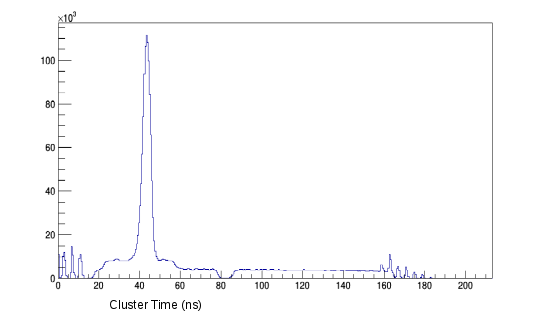
\includegraphics[width=0.5\textwidth]{t1.png}
  \caption{Cluster time in the readout window.}
\label{fig:ctime}
\end{figure}


The final time offset per crystal was the sum of the fine time offsets found using the RF signal and the gross 2 ns offset found by using two cluster events. 
\subsection{Time Walk}
After applying the time offsets to each crystal, a time walk correction was obtained by studying the time difference between hits in a cluster versus the seed hit as a function of the hit energy. The ultimate goal is to eliminate time walk over all hit energies as shown in \ref{fig:hitincluster}. 

\begin{figure}[H]
  \centering
      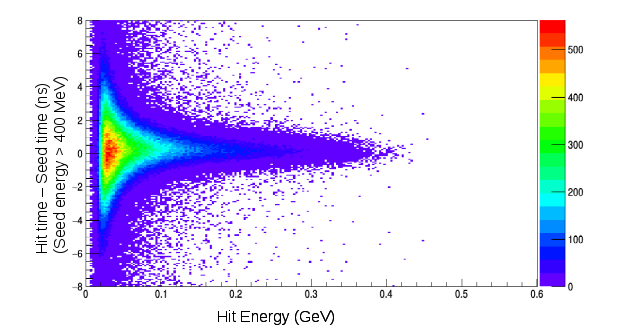
\includegraphics[width=0.5\textwidth]{hitIncluster_corr.png}
  \caption{Hit timing within clusters.}
\label{fig:hitincluster}
\end{figure}

The final time walk correction obtained from studying the timing of hits in a cluster shown in Figure \ref{fig:twalk}  shows that for crystal energies above 150 MeV, the time walk is not significant. While the time walk will not significantly affect the resolution of the two cluster time difference, the time walk is important in clustering in order to enable tighter cluster time cuts. \\
\begin{figure}[H]
  \centering
      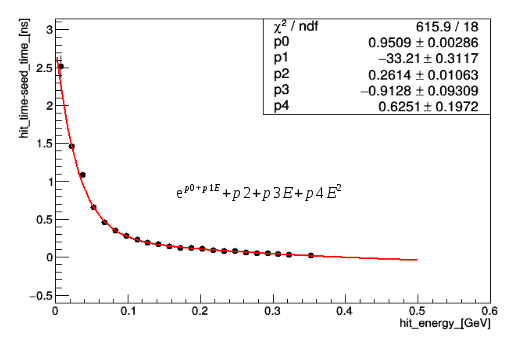
\includegraphics[width=0.5\textwidth]{twalk.png}
  \caption{Time walk correction for clusters where the seed hit energy is greater than 400 MeV.}
  \label{fig:twalk}
\end{figure}

%------------------------------------------------

\section{Results}
The time offsets found from the combination of studies using the RF signal and the two cluster timing are significant in reducing accidentals in two cluster event reconstruction. By comparing the energies of two clusters in two cluster events, there are two regions of particular interest in validating the calibration. The first region is the accidental region which can be seen in Figure \ref{fig:2clus} as the region where each cluster has an energy roughly equal to the beam energy which is kinematically forbidden to originate from the same physics event. The second region is the well-correlated event region. These well-correlated events come from trident production and M\o 1llers. This region has a cluster energy sum that is roughly equal to the beam energy and an energy difference of less than 200 MeV. \\ 
\begin{figure}[H]
  \centering
      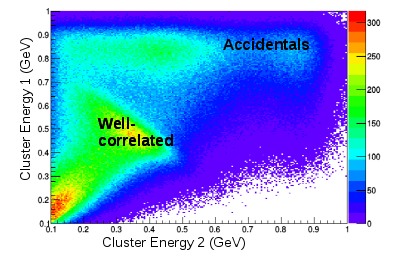
\includegraphics[width=0.5\textwidth]{2cluscolz.png}
  \caption{Two cluster energy distribution.}
\label{fig:2clus}
\end{figure}
By studying these events after applying the time offsets, one can observe that the time difference between two clusters in the accidental region occurs in increments of 2 ns with nearly equal likelihood as seen in the top of Figure \ref{fig:money}. This is in sharp contrast to the time difference of two well-correlated clusters where we observe only a single peak at zero with a width of approximately 480 ps. \\
\begin{figure}[H]
  \centering
      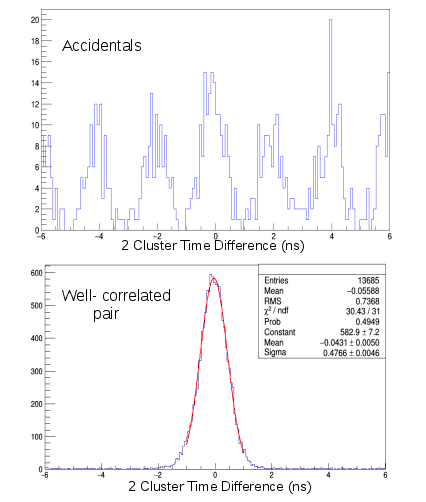
\includegraphics[width=0.5\textwidth]{2cluster.png}
  \caption{Two cluster resolution for correlated and accidental events.}
  \label{fig:money}
\end{figure}
After applying the time walk correction and time offsets, the hit timing within a cluster can also be used to study the timing resolution as a function of energy. For clusters with a seed energy greater than 450 MeV, the time difference of the hits within a cluster compared against the energy of the hits yields a time resolution as described by Equation \ref{eq:resolution} and shown in Figure \ref{fig:tresolution}.

\begin{equation}
\label{eq:resolution}
\textit{Time Resolution} = \dfrac{0.052}{E \textit{ (GeV)}}+0.2044 \textit{ ns}
\end{equation}

At the highest energies, derived from studying the resolution of the time difference between well-correlated pair clusters, the individual crystal resolution is approximately 340 ps.\\  
 \begin{figure}[H]
  \centering
      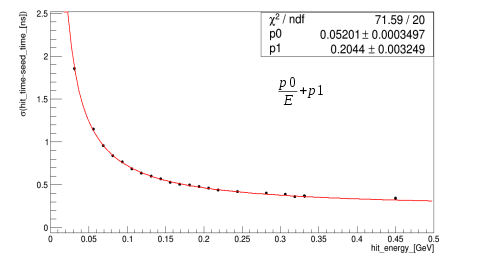
\includegraphics[width=0.5\textwidth]{tres1.png}
  \caption{ndividual crystal Ecal time resolution as a function of energy.}
\label{fig:tresolution}
\end{figure}

The final time offsets for the crystals in the Ecal can be seen in Figure \ref{fig:ecalOffsets}. One particular group has -4 ns time offsets and corresponds to a group of channels using a shorter readout cable from the Ecal to the FADC.  
 \begin{figure}[H]
  \centering
      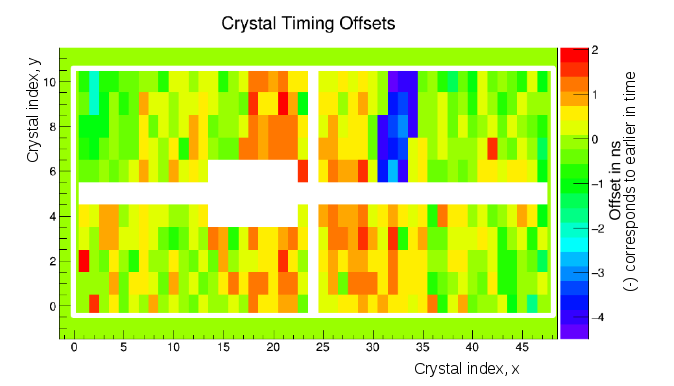
\includegraphics[width=0.5\textwidth]{ecalOffsets.png}
  \caption{Individual time offsets for each crystal.}
\label{fig:ecalOffsets}
\end{figure}


%------------------------------------------------

\section{Conclusion}

The results of this study enable improved timing resolution in the Ecal by finding time offsets for each crystal and a time walk correction that is more significant for lower energy hits and can improve timing cuts in clustering. The resultant time resolution for the Ecal, after applying the time walk correction and timing offsets, is small enough to significantly reduce accidental hits in clusters and accidentals clusters in events. All of the results in this note are implemented in the hps-java framework in EcalRawConverterDriver.java where the time offsets can be called from the conditions database, and the time walk can be applied. 

%----------------------------------------------------------------------------------------
%	REFERENCE LIST
%----------------------------------------------------------------------------------------

\begin{thebibliography}{99} % Bibliography - this is intentionally simple in this template

\bibitem{Kazimi} R. Kazimi,
\href{http://accelconf.web.cern.ch/accelconf/ipac2013/papers/thpfi091.pdf} Simultaneous Four-Hall Operation for 12 GeV CEBAF, Proceedings of IPAC 2013, Shanghai, China.

\bibitem{Baltzell} N. Baltzell,\href{https://confluence.slac.stanford.edu/download/attachments/192191938/3PoleAna.pdf?version=1&modificationDate=1434062944000&api=v2}
HPS Note 2015-010.
%Figueredo, A.~J. and Wolf, P. S.~A. (2009).
%\newblock Assortative pairing and life history strategy - a cross-cultural
%  study.
%\newblock {\em Human Nature}, 20:317--330. 
\end{thebibliography}

%----------------------------------------------------------------------------------------

\end{multicols}

\end{document}
